\documentclass[12pt]{article}

\usepackage{sbc-template}
\usepackage{graphicx,url}
\usepackage[utf8]{inputenc}
\usepackage[T1]{fontenc}
\usepackage[brazil]{babel}
\usepackage{booktabs}
\usepackage{tikz}
\usetikzlibrary{positioning,arrows.meta}

\sloppy

\title{OpiniON: previsão de conexões entre pessoas que se\\ encontram, a partir de uma pulseira de proximidade}

\author{João Pedro\inst{1}, Lucas Calabria\inst{1}, Maria Júlia Dantas\inst{1},
  Maria Luíza Dantas\inst{1},\\ Fábio André Oliveira Lins\inst{1},
  Marcus Vinicius Menezes Barbosa\inst{1}, Pedro Mota\inst{1},\\ Rodrigo Quirino de Mello\inst{1}}

\address{CESAR School -- Recife, PE -- Brasil
  \email{\{jpsa,lvc,mjdma,mldt,faol,mvmb,pom2,rqm\}@cesar.school}
}

\begin{document}

\maketitle

\begin{abstract}
  OpiniON is a social platform where people rate films, series, books, games and music. A wristband
  detects when two users are close to each other and the backend must decide whether to signal the
  encounter. We built the full machine learning pipeline that answers the question ``what is the
  chance that two people who just met will interact on the app within 48 hours?'': a virtual
  wristband publishing over MQTT, ingestion into PostgreSQL, an Airflow pipeline that computes
  leakage-free features, model comparison, Bayesian hyperparameter optimization and grouped
  cross-validation tracked in MLflow, and an inference service, API and dashboard deployed with Docker
  Compose. On a temporal test split, the optimized and calibrated AdaBoost model reaches a PR-AUC of
  0.188 among strangers (prevalence 0.014), against 0.131 for the taste-similarity rule.
\end{abstract}

\begin{resumo}
  O OpiniON é uma plataforma social em que as pessoas avaliam filmes, séries, livros, jogos e
  músicas. Uma pulseira detecta quando dois usuários estão próximos e o sistema precisa decidir se
  o encontro merece um sinal. Construímos o pipeline completo de aprendizado de máquina que responde
  à pergunta ``qual a chance de duas pessoas que acabaram de se encontrar interagirem no app em até
  48 horas?'': pulseira virtual publicando via MQTT, ingestão em PostgreSQL, pipeline no Airflow com
  features sem informação do futuro, comparação de modelos, otimização bayesiana e validação cruzada
  agrupada registradas no MLflow, além de serviço de inferência, API e dashboard implantados com
  Docker Compose. No teste temporal, o AdaBoost otimizado e calibrado alcança PR-AUC de 0,188 entre
  desconhecidos (prevalência de 0,014), contra 0,131 da regra de afinidade de gosto.
\end{resumo}

\section{Introdução}

Plataformas de recomendação costumam sugerir obras. O OpiniON propõe também sugerir pessoas, no
momento em que elas estão fisicamente próximas: no cinema, na livraria, no campus ou numa convenção
de jogos. A equipe de Design desenvolve uma pulseira que detecta a proximidade por Bluetooth e emite
sinais discretos (luz e vibração). A equipe de Ciência da Computação ficou responsável por decidir
\emph{quando} sinalizar.

Um sinal em excesso cansa o usuário e leva ao silenciamento da pulseira; um sinal ausente desperdiça
uma conexão. Por isso formulamos o problema como uma estimativa de probabilidade: dado um encontro
que acabou de terminar, qual a chance de os dois usuários interagirem no app (seguir, abrir o
perfil, curtir ou comentar uma avaliação, salvar uma obra avaliada pelo outro) nas 48 horas seguintes?
O público que importa são os \emph{desconhecidos}, pares em que nenhum dos dois segue o outro:
amigos interagem de qualquer forma e inflariam as métricas.

Este relatório descreve a solução entregue ao longo de nove requisitos (CC1 a CC9): dados e
infraestrutura de aquisição, pipeline, modelos, otimização, validação, integração, implantação e
visualização. O código está em \url{https://github.com/Lvcalabria06/opinion-ml}.

\section{Dados}

Não há usuários reais do OpiniON nem pulseira física. Para não inventar gostos, usamos a
\emph{Amazon Reviews 2023} \cite{hou2024bridging}: 1.200 usuários reais que avaliaram livros,
filmes, séries, jogos e música, com 48.018 obras e 58.251 avaliações (notas de 1 a 5, com gêneros).
Sobre esses usuários, um simulador gera 12 semanas de encontros (06/07 a 27/09/2026), seguidores e
interações no app, com quatro tipos de local e convenções de jogos nas semanas 3, 7 e 11.

O simulador decide as conexões por um processo probabilístico com variáveis ocultas (abertura social
de cada pessoa e compatibilidade ``verdadeira'') e ruído. Essas variáveis ficam numa pasta separada,
usada só para validação e nunca como \emph{feature}. Foram gerados 69.384 encontros, dos quais 8,1\%
terminaram em interação; entre desconhecidos, a taxa cai para cerca de 1,2\%. Todas as métricas deste
relatório medem, portanto, a mistura de gostos reais com encontros simulados, não o comportamento de
usuários reais da pulseira. Os testes do protótipo com pessoas (semana 16) devem refazer as
comparações com dados reais.

\section{Arquitetura da solução}

A Figura~\ref{fig:arquitetura} resume o fluxo. A pulseira virtual publica quatro tipos de mensagem
num broker MQTT (Mosquitto): \texttt{proximidade} no início do encontro, \texttt{encontro} no fim
(com duração e RSSI médio), \texttt{interesse} (toque do usuário) e \texttt{status} (modo de
descoberta). Os usuários aparecem como identificadores anônimos que mudam todo dia
(HMAC do usuário e da data com um segredo do servidor), e só o backend consegue traduzi-los.

\begin{figure}[ht]
\centering
\begin{tikzpicture}[
  caixa/.style={draw, rounded corners, align=center, font=\footnotesize, minimum height=0.9cm,
                minimum width=2.3cm, inner sep=3pt},
  seta/.style={-{Stealth[length=2mm]}, thick},
  rot/.style={font=\scriptsize, fill=white, inner sep=1pt}]
  \node[caixa] (pul) at (0,0) {Pulseira virtual};
  \node[caixa] (mqtt) at (3.4,0) {Broker MQTT};
  \node[caixa] (ing) at (6.8,0) {Ingestão};
  \node[caixa] (db) at (10.2,0) {PostgreSQL};
  \node[caixa] (inf) at (3.4,-2.1) {Consumidor de\\inferência};
  \node[caixa] (ml) at (6.8,-2.1) {MLflow};
  \node[caixa] (af) at (10.2,-2.1) {Airflow\\(pipeline + treino)};
  \node[caixa] (dash) at (3.4,-4.2) {Dashboard\\(Streamlit)};
  \node[caixa] (api) at (6.8,-4.2) {API\\(FastAPI)};
  \draw[seta] (pul) -- node[rot, above=2pt]{eventos} (mqtt);
  \draw[seta] (mqtt) -- (ing);
  \draw[seta] (ing) -- (db);
  \draw[seta] (db) -- node[rot, right=2pt]{dados} (af);
  \draw[seta] (af) -- node[rot, above=2pt]{registra} (ml);
  \draw[seta] (ml) -- node[rot, above=2pt]{modelo} (inf);
  \draw[seta] (mqtt) -- node[rot, right=2pt]{encontro} (inf);
  \draw[seta] (inf.west) -| node[rot, pos=0.75, left=2pt]{feedback} (pul.south);
  \draw[seta] (ml) -- node[rot, right=2pt]{modelo} (api);
  \draw[seta] (db.east) -- ++(0.5,0) |- node[rot, pos=0.75, below=2pt]{inferências e indicadores} (api.east);
  \draw[seta] (api) -- (dash);
\end{tikzpicture}
\caption{Arquitetura do OpiniON. Todos os serviços sobem com \texttt{docker compose up}.}
\label{fig:arquitetura}
\end{figure}

O serviço de ingestão valida cada mensagem contra o contrato, traduz os identificadores, confere se
a pulseira pertence ao usuário que publicou, deduplica as reentregas do QoS~1 e grava no banco. Na
\texttt{proximidade}, ele já calcula a afinidade de gosto do par por mídia e, se alguma passa do
corte, devolve à pulseira um aviso (``alguém por perto tem alta afinidade com você em música'').
Esse é o sinal imediato; o modelo atua no fim do encontro, quando duração e intensidade do sinal
Bluetooth já são conhecidas.

\section{Pipeline de dados e \emph{features}}

A DAG \texttt{opinion\_pipeline} do Apache Airflow tem sete tarefas: extração do banco para uma
área de \emph{staging}, cálculo da compatibilidade de gosto, das \emph{features} do encontro e do
rótulo (estas três em paralelo), preparação do conjunto de modelagem, resumo e treino do modelo de
produção. As mesmas funções são chamadas pela DAG, pelos experimentos e pelo serviço de inferência,
o que garante que o modelo em produção veja exatamente as \emph{features} com que foi treinado.

São 48 \emph{features} em cinco grupos: encontro (duração, RSSI, encontros anteriores do par),
contexto (local, período, dia da semana, modo discreto), compatibilidade (similaridade de gêneros,
concordância de notas, favoritas em comum, afinidade por mídia), perfil (atividade recente,
histórico, número de conexões) e relação (se já se seguem, se já interagiram). Toda \emph{feature}
usa apenas dados anteriores ao início do encontro. Um teste automatizado recalcula as
\emph{features} de 30 encontros apagando tudo o que aconteceu depois e exige resultado idêntico; o
mesmo teste falha quando um vazamento é inserido de propósito.

A divisão é temporal: treino nas semanas 1 a 8 (46.244 encontros), validação nas semanas 9 e 10
(10.101) e teste nas semanas 11 e 12 (11.970). Os 1.069 encontros do fim da semana 8 cujo rótulo
só seria conhecido na semana 9 são removidos do treino. Escolha de modelo, de hiperparâmetros e do
limiar acontece sempre na validação; o teste é medido uma única vez por modelo.

\section{Modelagem}

\subsection{Métrica e referência}

Com prevalência de cerca de 1,4\% entre desconhecidos no teste, a acurácia e a ROC-AUC dizem pouco.
A métrica de escolha é a área sob a curva precisão $\times$ revocação (PR-AUC) entre desconhecidos
\cite{saito2015precision}. Todo resultado é comparado com a \emph{regra simples}, que ordena os
encontros pela afinidade de gosto, e com o acaso (a prevalência). O limiar do sinal maximiza o
$F_{0,5}$, que pesa a precisão o dobro da revocação, porque um sinal errado custa mais do que um
sinal perdido.

\subsection{Comparação de modelos (CC3 e CC4)}

O \emph{baseline} explicável do CC3 foi uma regressão logística. No CC4 comparamos sete famílias no
mesmo protocolo, com grades pequenas e fixas \cite{pedregosa2011scikit}: regressão logística, árvore
de decisão, \emph{Random Forest}, \emph{Gradient Boosting}, KNN, AdaBoost e MLP. A
Tabela~\ref{tab:cc4} resume os resultados; os intervalos de confiança vêm de \emph{bootstrap}
pareado no teste.

\begin{table}[ht]
\centering
\caption{PR-AUC entre desconhecidos (CC4). Escolha na validação; teste medido uma vez.}
\label{tab:cc4}
\footnotesize
\begin{tabular}{lccc}
\toprule
Modelo & Validação & Teste (IC 95\%) & Brier (teste) \\
\midrule
AdaBoost (escolhido) & 0,136 & 0,186 (0,148--0,246) & 0,088 \\
Gradient Boosting & 0,130 & 0,176 (0,139--0,228) & 0,061 \\
Random Forest & 0,128 & 0,184 (0,145--0,239) & 0,060 \\
Árvore de decisão & 0,116 & 0,156 (0,125--0,195) & 0,066 \\
MLP & 0,107 & 0,139 (0,106--0,189) & 0,062 \\
Regressão logística & 0,101 & 0,159 (0,120--0,223) & 0,147 \\
KNN & 0,060 & 0,101 (0,073--0,153) & 0,061 \\
Regra simples & 0,100 & 0,131 (0,104--0,177) & -- \\
Acaso & -- & 0,014 & 0,073 \\
\bottomrule
\end{tabular}
\end{table}

Os modelos de conjunto ficam à frente, mas próximos entre si: os intervalos se sobrepõem e a
diferença do AdaBoost para a regressão logística (+0,027) tem intervalo que inclui zero. Contra a
regra simples, a vantagem é consistente (+0,055, IC 95\% de +0,015 a +0,099). No limiar escolhido,
o AdaBoost acerta 24,1\% dos sinais, contra 18,8\% da regra, sinalizando a mesma fração de encontros.
O KNN fica atrás porque as \emph{features} são heterogêneas e a distância euclidiana trata todas
como igualmente importantes. A probabilidade escondida do simulador, que nenhum modelo pode usar,
alcança PR-AUC de 0,396: a distância até ela vem do que os dados não observam (a abertura social
de cada pessoa) e do sorteio do resultado.

\subsection{Otimização de hiperparâmetros (CC5)}

Otimizamos o AdaBoost com otimização bayesiana pelo Optuna (amostrador TPE)
\cite{akiba2019optuna}, em 30 tentativas, e rodamos uma busca aleatória com o mesmo orçamento como
controle. As duas começam pela melhor configuração da grade do CC4, então nenhuma termina pior que
ela na validação. Cada tentativa virou um \emph{run} no MLflow \cite{zaharia2018accelerating}.

O TPE chegou a PR-AUC de 0,150 na validação ($n\_estimators=292$, taxa de aprendizado 0,94, tocos
de profundidade 1), a busca aleatória a 0,148 e a grade a 0,136 (Figura~\ref{fig:cc5}). A taxa de
aprendizado explicou 90\% da variação entre tentativas. No teste, o modelo otimizado ficou em 0,188
(IC 95\% de 0,146 a 0,248), praticamente igual ao da grade (+0,001): o ganho na validação reflete
em boa parte a seleção entre muitas tentativas no mesmo conjunto. Depois da busca, calibramos as
probabilidades com uma sigmoide ajustada na validação \cite{platt1999probabilistic}. Por ser
monótona, ela não altera a ordenação, mas reduziu o Brier no teste de 0,101 para 0,063, o que
permite exibir a saída como chance na API e no dashboard.

\begin{figure}[ht]
\centering
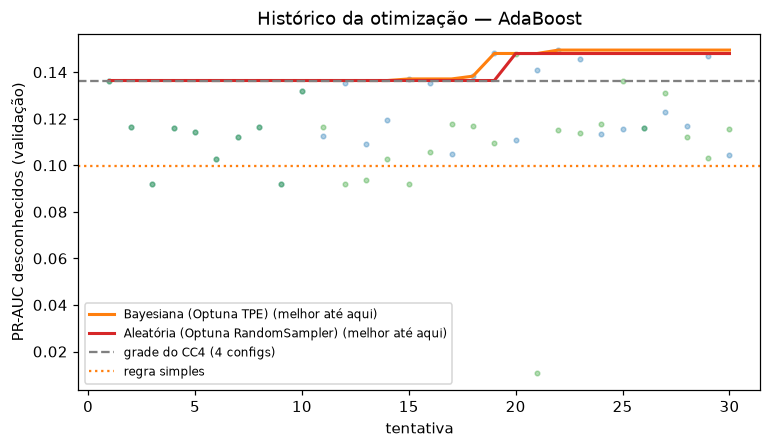
\includegraphics[width=.75\textwidth]{figuras/historico.png}
\caption{Histórico da otimização: melhor PR-AUC na validação até cada tentativa.}
\label{fig:cc5}
\end{figure}

\subsection{Validação cruzada, estabilidade e generalização (CC6)}

Avaliamos o modelo otimizado com \emph{stratified k-fold} agrupado por par ($k=5$, grupo = par de
usuários) nas semanas 1 a 10, sem tocar no teste. O agrupamento impede que um par seja avaliado
depois de ter sido visto no treino. A PR-AUC entre desconhecidos foi $0{,}139 \pm 0{,}011$
(coeficiente de variação de 8\%), contra $0{,}084 \pm 0{,}010$ da regressão logística e
$0{,}109 \pm 0{,}021$ da regra, que o modelo superou em quatro dos cinco folds
(Figura~\ref{fig:cc6}). A variação entre partições é baixa.

\begin{figure}[ht]
\centering
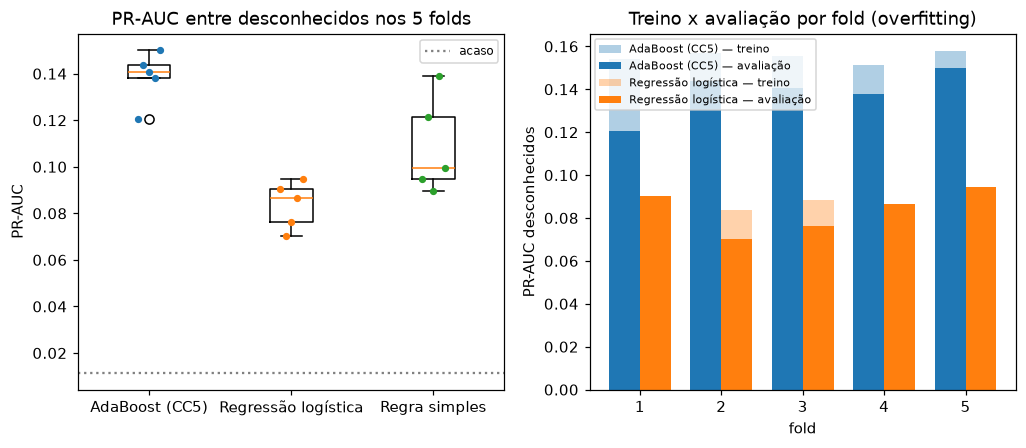
\includegraphics[width=\textwidth]{figuras/folds.png}
\caption{Validação cruzada agrupada por par: dispersão por fold e treino $\times$ avaliação.}
\label{fig:cc6}
\end{figure}

No treino de cada fold, o AdaBoost tem PR-AUC de 0,155, 11,8\% acima da avaliação: há algum
sobreajuste, mas sem memorização forte. A curva de aprendizado se estabiliza a partir de metade do
treino (0,132 com 50\% e 0,135 com 100\%), e treino e avaliação convergem: mais encontros simulados
do mesmo tipo trariam pouco ganho, e o limite está na informação disponível nas \emph{features}. A
regressão logística quase não sobreajusta (0,5\%), mas fica bem abaixo, um sinal de viés.

Como o k-fold mistura semanas, complementamos com uma janela temporal expansível: treinando nas
semanas anteriores e avaliando a semana seguinte, o modelo ficou entre 0,102 e 0,177 (média 0,151)
nas semanas 5 a 10. O desempenho se mantém quando o modelo prevê semanas que não viu. O valor do
teste (0,188) fica acima da faixa dos folds, o que é coerente com a prevalência maior nas semanas 11
e 12, que incluem uma convenção de jogos.

\section{Integração, implantação e visualização}

\textbf{Inferência (CC7).} Um consumidor assina os tópicos \texttt{encontro}, traduz os
identificadores, calcula as \emph{features} com as mesmas funções do pipeline (só com o passado do
encontro) e estima a chance com o modelo de produção do MLflow. O resultado é gravado no banco e,
se a chance passa do limiar, o sinal volta à pulseira pelo tópico \texttt{feedback}, em duas faixas
(leve a partir do limiar, perceptível a partir de 1,5 vez o limiar). Pulseiras em modo pausado não
recebem sinal. Cada encontro é pontuado em menos de um segundo. Uma API (FastAPI) expõe a mesma
inferência, recebendo o encontro no formato do contrato MQTT, e fornece os dados do dashboard. A
última tarefa da DAG reajusta a configuração otimizada com os dados novos, recalibra, e só promove a
nova versão se ela superar a regra simples na validação; API e consumidor recarregam o modelo
sozinhos.

\textbf{Implantação (CC8).} Um único \texttt{docker compose up} sobe broker, banco, carga do
histórico, ingestão, pulseira (reprodução das 12 semanas e depois encontros ao vivo), servidor
MLflow com proxy de artefatos, Airflow, consumidor de inferência, API, dashboard e um visualizador
do banco. Validamos o fluxo de ponta a ponta com os mesmos serviços configurados como no
\emph{compose}: 69.384 encontros chegaram ao PostgreSQL sem perdas, a DAG executou as sete tarefas e
registrou o modelo no servidor MLflow, e os encontros gerados ao vivo foram pontuados
automaticamente.

\textbf{Dashboard (CC9).} Em Streamlit, mostra os encontros e as inferências em tempo real, os
sinais emitidos, as métricas do modelo servido e os indicadores de produto: taxa de conversão dos
encontros (8,1\%), precisão do aviso de afinidade (14,5\% dos encontros avisados converteram) e
taxa de silenciamento, isto é, sinais seguidos de pausa da pulseira em até 24 horas.

\section{Limitações}

O rótulo é simulado: a ordem entre modelos próximos, a importância das \emph{features} e os
hiperparâmetros ótimos dependem das premissas do simulador e não devem ser apresentados como
descobertas sobre pessoas. A validação do simulador encontrou uma taxa de interação entre
desconhecidos (1,2\%) abaixo da faixa considerada plausível. Nos recortes por mídia com poucos
encontros (jogos e séries), a escolha do modelo na validação não se sustentou no teste, por isso a
solução usa o modelo geral. A validação, usada para escolher hiperparâmetros, calibração e limiar, é
a mesma, o que deixa a estimativa de validação otimista; o teste e a janela temporal mostram a
diferença. Por fim, a execução do \texttt{docker compose} com a construção das imagens precisa ser
repetida num ambiente com acesso ao Docker Hub.

\section{Conclusão}

Entregamos uma solução completa e reproduzível, da pulseira ao dashboard, em que o modelo é
treinado, otimizado, validado e servido com as mesmas funções de \emph{features} e com o protocolo
temporal preservado em todas as etapas. O modelo supera a regra de afinidade de gosto de forma
consistente no teste, nos folds e nas semanas futuras, e as probabilidades calibradas permitem
sinais em faixas. O próximo passo é substituir os encontros simulados pelos dados dos testes do
protótipo do Design com pessoas reais, refazer a comparação e definir com o Design o custo de um
sinal errado, que determina o limiar.

\bibliographystyle{sbc}
\bibliography{referencias}

\end{document}
